\documentclass{article}

\usepackage[utf8]{inputenc}
\usepackage{amsmath}
\usepackage{amsfonts}
\usepackage[numbers]{natbib}
\bibliographystyle{plainnat}
\usepackage{url} % insert Urls in bib	
\usepackage{amsthm} % For proofs
\usepackage{tikz} % images

\newtheorem{definition}{Definition}
\newcommand{\rnums}{\mathbb{R}}

\title{Convex v.s. Non-Convex Problems}
\author{Gerardo Durán Martín}
\begin{document}
	\maketitle
	
	All throughout science, the search for an optimal solution is often presented as an approximation of reality. Be it to fit a curve for a given set of points that make an interest rate curve in quantitative finance; to find the optimal path in operations research; or the study of equilibrium under an economic model, to say a few. Solving these problems lead to the understanding of reality and optimal decision taking given the information available.\\
	
	Interestingly enough, how these problems are solved are as important as the problems themselves, the same algorithm might yield a different representation depending on the \textit{structure} of the problem. This structure becomes essential in high-dimensional spaces, where there is no clear graphical representation of the problem at stake.\\
	
	In this essay, which I declare is my own personal work, we will discuss about this structural property in the context of machine learning: a subject whose foundation lies in solving a collection of problems coming from both spectrums.\\
	
	 The \textit{problem} in machine learning, is to make sense of the information available and generalize what has been \textit{learned} to a unseen (out of training) dataset. \textit{Learning}, in this sense, is the ability to extract information from data.\\
	
	To solve the learning problem, we need a way to quantify how much information the model was able to attain during its training phase. In parametric regression problems, for example, the main goal is to find a set of parameters $\theta$ to a function $g:\rnums^n\to\rnums^m$ that best approximates an input vector $X\in\rnums^n$ to an output vector $y\in\rnums^m$. In this sense, we would like to find $\theta$ such that $g(X|\theta) \approx y$. To determine how significant the approximation to $y$ given $\theta$ is, we introduce the loss function $J: \rnums^m \to \rnums$ whose goal is to measure the difference between the model and the observed points; the smaller $J$ is, the better the approximation. The search for an optimal solution to to $J$ is regarded as an optimization problem, and its solution, $\theta^*$, is such that	
	\begin{equation}\label{eq:opt_solution}
		\theta^* = \text{argmin}_\theta  J(\theta).
	\end{equation}
	
	If the parameter $\theta^*$ is such that for every other $\theta$, $J(\theta^*) \leq J(\theta)$, then we say that $\theta^*$ is a global minimum. If, on the other hand, $\theta^*$ is such that $J(\theta^*) \leq J(\theta)$ for every $\theta \in$ $\{\hat\theta \ | \  ||\hat\theta - \theta^*|| < \epsilon\}$ with $\epsilon > 0$, we say that $\theta^*$ is a local minimum. It is then, that to find the global minimum in $J$ is to find the value that guarantees the optimal solution for the problem in question (see eq. \ref{eq:opt_solution}) . How, then, can one guarantee to have found a global minimum or even assert its existence? A crucial consideration is to know whether the problem is \textbf{convex or non-convex}.\\
		
	On a superficial level, we regard a convex functions as smooth and \textit{well behaved}. To understand this, consider the definition of a convex function.
	
	\begin{definition}[Convex Function]
		A function $f:\rnums^n \to \rnums$ is said to be convex if the domain of $f$ is convex and, if for every $x_1$, $x_2$ $\in D_{f}$, $\alpha \in [0, 1]$,
		\begin{equation}
 			f(\alpha x_1 + (1-\alpha)x_2) \leq \alpha f(x_1) + (1 - \alpha) f(x_2).
		\end{equation}
	\end{definition}
	
	For a function $f: \rnums \to \rnums$, the definition of a convex function is akin to a line passing from $f(x_1)$ to $f(x_2)$ that is above or at the same level as the image of $f$ between $x_1$ and $x_2$. This last fact guarantees the existence of a global minimum (see \cite{boyd}) . In light of the former, it might seem desirable to work with convex problems and, in some cases, transform the optimization problem as that in which the function to minimize is convex. In fact, this was the case for many years, so much so that extensive books exist on the matter, whose analysis and resolution is still relevant. As problems grew complex, \cite{Jain-Kar} points, researchers looked for ways to transform seaming non-convex problems into convex. Even though said transformations were made possible, research has shown that solving the non-convex form for some of these problem offer more scalable solutions.\\
	
	\begin{figure}
		\centering
		\includegraphics[width=0.8\textwidth]{conv_nonconvR2}
		\caption{Comparison between a convex and non-convex function. \textit{Left}: the convex function $f(x) = x^2$. For any $x_1 < x_2$, the line $\{\alpha x_1^2  + (1 - \alpha) x_2^2 \ | \ \alpha \in [0,1]\}$ is always above or at the same level as $\{(\alpha x_1  + (1 - \alpha) x_2)^2 \ | \ \alpha \in [0,1]\}$; \textit{Right}: The non-convex function $f(x) = \sin(x^2)$. Considering $\alpha = 0.2$, and $x_1 = \pi / 2$. $x_2 = 10 \pi / 16$, $\sin(\alpha x_1 + (1 - \alpha) x_2)^2 = 1 > \alpha \sin(x_1 ^ 2) + (1 - \alpha) \sin(x_2^2) \approx -0.3989$.}
		\label{fig:conv_nonconvr2}
	\end{figure}
		
	To understand the phenomenon of convexity in machine learning, let us consider a toy example contrasting two key models, that of linear regression and single hidden-layer neural network with sigmoid activation function and a linear output. We consider the training dataset $X\in\rnums^{m\times n}$, $y\in\rnums^{1\times n}$ with $n$ training points and $m$ input parameters, where $\{X_{i,j}\}_{i,j}$, $\{y_{i,j}\}_{i,j} \sim N(0,1)$ and $L_2$ loss function $J(\cdot) = \frac{1}{2} ||g(X|\cdot) - y||_2$.\\
		
	For the linear regression model we assume existence of a linear relationship between $X$ and $y$. The aim is to find $\theta\in\rnums^{m}$ that models $g(X|\theta) = \theta^T X$ and minimizes $J$. Under this setting, $J$ is a convex function of $\theta$. To show this, we must prove that $J(\alpha \theta_1 + (1 - \alpha)\theta_2) \leq \alpha J(\theta_1) + (1 - \alpha)J(\theta_2)$, $\forall \  \theta_1, \theta_2 \in \rnums^{m}$, $\alpha \in [0,1]$.
	
	\begin{proof}
	\begin{align*}
		&J(\alpha \theta_1 + (1 - \alpha)\theta_2) \\
		&= ([\alpha \theta_1 + (1 - \alpha)\theta_2]^TX -y)([\alpha \theta_1 + (1 - \alpha)\theta_2]^TX -y)^T\\
		&= ([\alpha \theta_1 + (1 - \alpha)\theta_2]^TX -y)(X^T[\alpha \theta_1 + (1 - \alpha)\theta_2] -y^T)\\
		&= [\alpha\theta_1 + (1-\alpha)\theta_2]^TXX^T[\alpha\theta_1 + (1-\alpha)\theta_2] - 2[\alpha\theta_1 + (1-\alpha)\theta_2]^TXy^T + yy^T\\
		&\text{Where, by Jensen's Inequality, considering the quadratic function $f(\theta) = \theta^TXX^T\theta$,}\\
		&\leq \alpha \theta_1^TXX^T\theta_1 + (1 - \alpha) \theta_2^TXX^T\theta_2 - 2[\alpha\theta_1 + (1-\alpha)\theta_2]^TXy^T + yy^T\\
		&= \alpha(\theta_1^TXX^T\theta_1 - 2\theta_1^TXy^T + yy^T) + (1 - \alpha)(\theta_2^TXX^T\theta_2 - 2\theta_2^TXy^T + yy^T) \\
		&= \alpha(\theta_1^TX - y)(\theta_1^TX - y)^T + (1 - \alpha)(\theta_2^TX - y)(\theta_2^TX - y)^T\\
		&= \alpha ||\theta_1^TX - y||_2 + (1 - \alpha) ||\theta_2^TX - y||_2
	\end{align*}
	\end{proof}
	
	\begin{figure}[h!]
		\centering
		\includegraphics[width=0.7\textwidth]{lreg_loss}
		\caption{Linear regression loss surface.}
		\label{fig:convex_loss}
	\end{figure}
	
	
	Graphically, this implies that the image for $J$, as a function ofz $\theta$, is an $m + 1$ dimensional bowl-like surface. Figure \ref{fig:convex_loss} shows the loss surface $J$ considering the third and fourth parameters in a linear regression with $n=1000$ and $m=10$.\\
	
	Let us now analyze the loss function for a neural network architecture. As stated by \cite{vidal-et-al}, the rise in neural network research and application has been largely due the availability of massive datasets, and efficient GPU computing hardware. Many of the mathematical reasons behind deep neural networks remain a mystery, yet this has not stop the application and engineering efforts to come up with evermore clever and complex ways to develop these architectures.\\
	
	Deep neural networks are non-convex in nature. To graphically analyze this property, let us now consider the neural network architecture proposed. The output for this neural network is $g(X|W^{[1]}, W^{[2]}) = W^{[2]}\sigma\left(W^{[1]} X\right)$, where $\sigma(x) = 1 / (1 + e^{-x})$ is applied element-wise. Consider $W^{[1]} \in \rnums^{4\times 10}$, $W^{[2]} \in \rnums^{1\times 4}$ initialized randomly as gaussian noise, the grid shown in figure \ref{fig:nonconvex_loss} represents the surface of $J$ as a function of two parameters, leaving the rest constant. Under this setting, the surface is non-smooth, contrary to the loss surface seen in the linear model.\\
		
	\begin{figure}[h!]
		\centering
		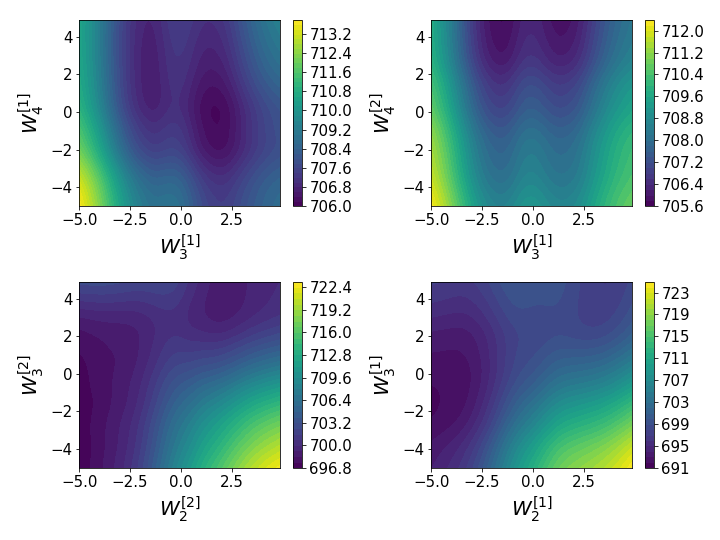
\includegraphics[width=0.8\textwidth]{nnet_loss}
		\caption{Neural Network Loss Surface}
		\label{fig:nonconvex_loss}
	\end{figure}
	
	
	As we can see, knowing the structure of the problem, being convex or non-convex, hints at at the sort of problems, or advantages, one might encounter in solving it. For some models, as  the linear regression with $m < n$, there exists a closed form solution known as the \textit{normal equation} that yields the global minimum. Some problems nowadays, however, have too much data to fit into memory and solve in closed form solution, or the algorithms to solve them have no closed form solution. In machine learning and neural networks, gradient descent and its variation like ADAM, RMSProp or Mini-batch Gradient Descent are the current algorithms of choice to approximate a local minimum.\\
	
	At the spirit of this powerful algorithm lies a rather intuitive and simple to implement idea. Given a loss function $J$, and a vector $\theta$ of parameters, the idea is to gradually reach a local minimum by computing the gradient of the loss function with respect to every parameter in the model and decrease at a rate $\alpha$ to the direction of steepest descent.  
	\begin{equation}
		\theta_i :=\theta_i - \alpha \frac{\partial}{\partial \theta_i} J(\theta) \ \forall \ i \in \{1 \ldots, m\},
	\end{equation}
	
	Gradient descent can be applied to both convex and non-convex problems, although knowing that $J$ is a convex function of $\theta$ guarantees, as we have seen, to reach a global minimum. The downside of gradient descent and its variations are the selection of the hyperparameters and, for non-convex problems, we can only guarantee local convergence.\\
	
	The growing research in non-nonvex problems, the quintessential example in machine learning being neural networks, brings about a whole new area of research to further expand our understanding in the subject. Significant proposals, such as the one made by Geoffrey Hinton \cite{levine}, invite to even redesign the most important algorithm to learn neural network parameters: backpropagation. \\
	
	The consequences from understanding these problems, although theoretical, bear important presence in applied settings as well. In the age of big data, a vast amount of information is useless without the power to abstract knowledge.
	
	
	\begin{figure}
		\centering
		\includegraphics[width=0.8\textwidth]{graddesc}
		\caption{Gradient Descent Hyperparameter selection. We consider the function $f(x) = x^2$ to test the effects of gradient descent. \textit{Left}: The learning rate is to big and the gradient shoots upwards. \textit{Right}: The learning rate is to small, convergence will take a considerable amount of iterations before reaching the minimum.}
		\label{fig:graddesc}
	\end{figure}
	
\nocite{*}
\bibliography{ref}
\end{document}